\section{Methodology}
This section deals with: design considerations, position, velocity and acceleration analysis of the Stewart platform. Both kinematic analysis and dynamic analysis will be looked at.

\subsection{Stewart Platform}
\subsubsection{Design Considerations}
\begin{enumerate}
\item When the controllable axes are active, the platform must be controlled in six degrees of motion.
\item When the controllable members are stationary the
platform must have a corresponding fixed position.
\item The mechanism should be light.
\item Velocity and position control of the mechanism should be easy to achieve.
\end{enumerate}
\subsubsection{Kinematic Analysis}


\subsection{Force Sensor}
\paragraph{}The force sensor module will be used to measure the force and moments from the aerodynamic loads applied on model being tested in the wind tunnel. The forces to be measured are the drag, lift and thrust as well as associated moments. For this subsystem two possible conceptual designs are to be considered:
\begin{itemize}
\item External force sensor
\item Stewart Platform as a force sensor
\end{itemize}
\subsubsection{External Force Sensor}
\paragraph{}In this case it would require at least 3 orthgonally positioned load cells measuring each force component. Each load cell would be mechanically linked to the model such that forces experienced on each axis are measured by each load cell. 
\begin{center}
	\begin{figure}[!h]
		\centering
		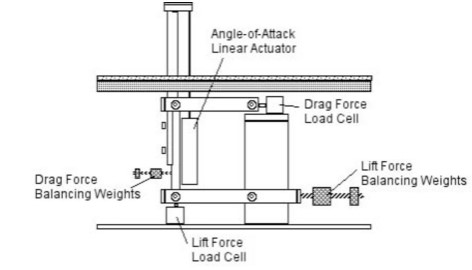
\includegraphics{Figures/modBal}
		\caption{Diagram of a force balance \cite{post_force_2010}}
	\end{figure}
\end{center}
\paragraph{} This configuration is however bulky by requiring an additional external system for force measurements in addition to the stewart platform for positioning the model. This is however complemented by the simplicity in calibration of the load cells and does not require a complex force transformation matrix and other issues with force amplification created by the use of an integrated system.
\subsubsection{Stewart Platform as a force sensor}
\paragraph{} In this configuration the stewart platform legs are used as force sensors by attaching strain gauges in the legs of platform. Similar work has been done by \cite{ferreira2015design} without the use of actuators as is proposed in this project. Using the stewart platform as a force sensor requires the actuators to be locked with zero degrees of freedom.
\paragraph{} Four strain gauges are required for each leg for a full wheatstone bridge configuration. 
\begin{center}
	\begin{figure}[!h]
		\centering
		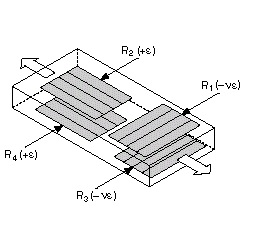
\includegraphics{Figures/loadConf}
		\caption{Strain Gauge Configuration \cite{noauthor_measuring_nodate}}
	\end{figure}
\end{center}
\paragraph{}In this case as shown in the figure the load cells are able to measure the axial strain on each leg. R1 and R3 are active strain gauges measuring the compressive Poisson effect (–νe). R2 and R4 are active strain gages measuring the tensile strain (+e). The output generated from the wheatstone bridge is then amplified and read to determine the strain on each leg.
\paragraph{Force transformation matrix}
In such a case the forces experienced at the top of the platform are distributed between the 6 legs and as result, a force transformation matrix is required to resolve the forces apllied on each axis as measured by each load cell on each leg. 
\paragraph{} If the platform is acted upon by an external wrench {$\vec{F}_e, \vec{M}_e$}, for static equilibrium of the body, the external wrench is statically balanced by the six leg forces of the stewart platform. Representing the unit vector $\hat{I}_i$ along the i-th leg with respect to B, the leg force is given  by $\hat{I}_if_i$. Considering the force equilibrium of the platform along  three mutually perpendicular directions in B(XYZ), the following force equations can be obtained:
\paragraph{}$(F_e)_x = f_1I_{1x} + f_2I_{2x} + f_3I_{3x} + f_4I_{4x} + f_5I_{5x} + f_6I_{6x}$
\paragraph{}$(F_e)_y = f_1I_{1y} + f_2I_{2y} + f_3I_{3y} + f_4I_{4y} + f_5I_{5y} + f_6I_{6y}$
\paragraph{}$(F_e)_z = f_1I_{1z} + f_2I_{2z} + f_3I_{3z} + f_4I_{4z} + f_5I_{5z} + f_6I_{6z}$
\paragraph{} where $(F_e)_x$, $(F_e)_y$ and $(F_e)_z$ are the external forces on the platform along three mutually perpendicular directions x, y and z of the frame B, respectively.
\paragraph{} The moment due to the forces $\hat{I}_if_i$ about the origin of B is $(\vec{b}_i x \hat{I}_i)f_i$. Considering the moment equilibrium about x, y and z axes of B, the following moment equations can be obtained:
\paragraph{}$(M_e)_x = f_1(\vec{b}_1 x \hat{I}_1)_x + f_2(\vec{b}_2 x \hat{I}_2)_x + f_3(\vec{b}_3 x \hat{I}_3)_x + f_4(\vec{b}_4 x \hat{I}_4)_x + f_5(\vec{b}_5 x \hat{I}_5)_x + f_6(\vec{b}_6 x \hat{I}_6)_x$
\paragraph{}$(M_e)_y = f_1(\vec{b}_1 x \hat{I}_1)_y + f_2(\vec{b}_2 x \hat{I}_2)_y + f_3(\vec{b}_3 x \hat{I}_3)_y + f_4(\vec{b}_4 x \hat{I}_4)_y + f_5(\vec{b}_5 x \hat{I}_5)_y + f_6(\vec{b}_6 x \hat{I}_6)_y$
\paragraph{}$(M_e)_z = f_1(\vec{b}_1 x \hat{I}_1)_z + f_2(\vec{b}_2 x \hat{I}_2)_z + f_3(\vec{b}_3 x \hat{I}_3)_z + f_4(\vec{b}_4 x \hat{I}_4)_z + f_5(\vec{b}_5 x \hat{I}_5)_z + f_6(\vec{b}_6 x \hat{I}_6)_z$
where $(M_e)_x$, $(M_e)_y$ and $(M_e)_z$ are the external moments on the platform  about the three coordinate axes of B. Combining the equations the relationship between the external wrench and the forces experienced by the legs can be expressed as follows:
$$
\begin{Bmatrix}
\vec{F}_e \\
\vec{M}_e \\
\end{Bmatrix} = [H]\{F\}
$$

\subsection{Velocity Measurement}
An important part in wind tunnel measurements is the measure of pressure at specific points in the wind tunnel and computing the correspondingair speed. This is achieved by the use of a pitot probe. 
\begin{center}
\begin{figure}
\centering
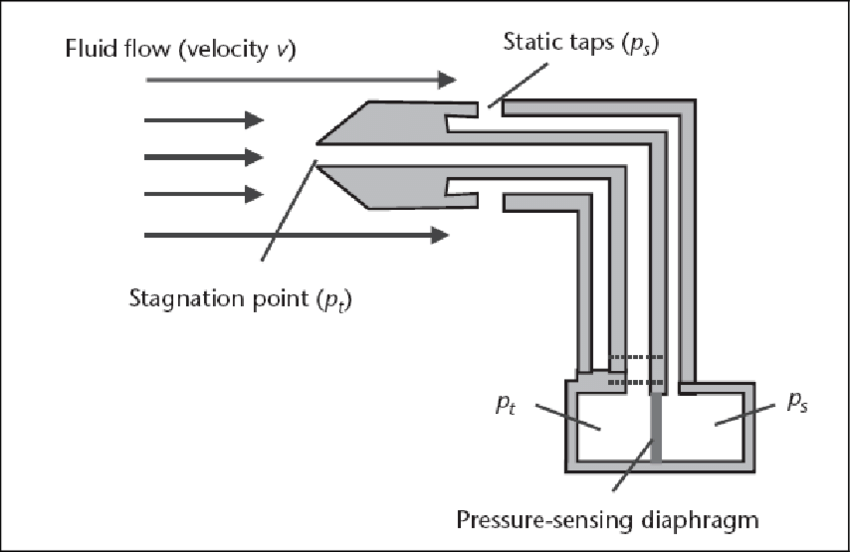
\includegraphics{Figures/pitot}
\caption[Pitot-static tube]{Pitot-static tube \cite{noauthor_wind_nodate}}
\end{figure}
\end{center}

The equation relates the speed of the fluid at a point to both the mass density of the fluid and the pressures at the same point in the flow field. For steady flow of an incompressible fluid for which viscosity can be neglected, the fundamental equation has the form:

$$ v = \sqrt{\frac{2(P_0 - P)}{\rho}}$$

Where V is the speed of the fluid, P0 is the total, also called the stagnation, pressure at that point of measurement, and p is the static pressure at the same point.

Three pitot probes are to be used in the wind tunnel, these are in the test section, intake and dissuser sections.